\tikzstyle{input_neuron}=[circle,draw=red!50,fill=red!10,thick,minimum size=6mm]
\tikzstyle{hidden_neuron}=[circle,draw=blue!50,fill=cyan!10,thick,minimum size=6mm]
\tikzstyle{output_neuron}=[circle,draw=green!50,fill=green!10,thick,minimum size=6mm]

\tikzstyle{input}=[circle,draw=black!50,fill=black!20,thick,minimum size=6mm]

\begin{center}
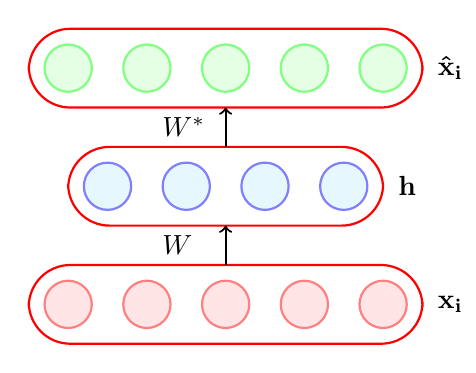
\begin{tikzpicture}

\node [input_neuron] (neuron01) at (6.5,4.5) {};
\node [input_neuron] (neuron02) at (7.5,4.5){};
\node [input_neuron] (neuron03) at (8.5,4.5) {};
\node [input_neuron] (neuron04) at (9.5,4.5) {};
\node [input_neuron] (neuron05) at (10.5,4.5) {};
\node [hidden_neuron] (neuron51) at (7,6) {} ;
\node [hidden_neuron] (neuron52) at (8,6)  {};
\node [hidden_neuron] (neuron53) at (9,6)  {};
\node [hidden_neuron] (neuron54) at (10,6)  {};

\node [output_neuron] (neuron11) at (6.5,7.5)  {};
\node [output_neuron] (neuron12) at (7.5,7.5)  {};
\node [output_neuron] (neuron13) at (8.5,7.5)  {};
\node [output_neuron] (neuron14) at (9.5,7.5)  {};
\node [output_neuron] (neuron15) at (10.5,7.5)  {};

\node[text width=0.01cm] at (11.2,4.5) {$\mathbf{x_i}$};
\node[text width=0.007cm] at (7.7,5.25) {$W$};
\node[text width=0.01cm] at (10.7,6) {$\mathbf{h}$};
\node[text width=0.007cm] at (7.7,6.75) {$W^*$};
\node[text width=0.01cm] at (11.2,7.5) {$\mathbf{\hat{x}_i}$};

\draw[red!100,thick,solid,rounded corners=15pt] (6,4) rectangle (11,5);
\draw[red!100,thick,solid,rounded corners=15pt] (6.5,5.5) rectangle (10.5,6.5);
\draw[red!100,thick,solid,rounded corners=15pt] (6,7) rectangle (11,8);



\draw[thick,->] (8.5,5) -- (8.5,5.5);

\draw[thick,->] (8.5,6.5) -- (8.5,7);



\end{tikzpicture}
\end{center}
